\documentclass[12pt,a4paper]{article}

\usepackage[utf8]{inputenc}
\usepackage[T2A]{fontenc}
\usepackage[ukrainian]{babel}

\usepackage{geometry}
\geometry{left=2cm,right=2cm,top=2cm,bottom=2cm}
\usepackage[table]{xcolor}
\usepackage{graphicx}
\usepackage{placeins}
\usepackage{array,multirow}
\usepackage{booktabs}
\usepackage{caption}
\renewcommand{\thetable}{№\arabic{table}}
\renewcommand{\thefigure}{\arabic{figure}}
\captionsetup[table]{name=Таблиця}

\usepackage{amsmath}
\usepackage{pdflscape}
\usepackage{hyperref}

\usepackage{subcaption}

\usepackage{minted}

\usemintedstyle{vs}
\setminted{linenos, breaklines, frame=single, fontsize=\small}

\begin{document}

    \begin{titlepage}

        % Картинка шапки (по центру, з відступом від верху)
        \begin{center}
\includegraphics[width=0.7\textwidth]{../../../TITLES/letterhead.png}\end{center}

        \begin{center}
            \large Національний технічний університет України\\
            «Київський політехнічний інститут імені Ігоря Сікорського»\\[1em]
            Факультет інформатики та обчислювальної техніки\\
            Кафедра обчислювальної техніки
        \end{center}

        \vfill

        \begin{center}
            \textbf{\LARGE Практична електроніка}\\[2em]
            \textbf{\Large Лабораторна робота №8}\\[0.5em]
            «Реалізація транзисторних ключів для Arduino»
        \end{center}

        \vfill

        \begin{flushright}
            Виконав: студент 2 курсу ФІОТ, гр. ІО-41\\
            \textit{Давидчук А.~М.}\\[1em]
            Перевірив: \textit{Гайдай А.~Р.}
        \end{flushright}

        \vfill

        \begin{center}Київ --- 2025\end{center}

    \end{titlepage}

    % Основний документ:

    \setlength{\parindent}{1.5em}

    \textbf{\underline{Тема:}} «Реалізація транзисторних ключів для Arduino».
    
    \vspace{1em}

    \textbf{\underline{Мета:}} реалізувати транзисторні ключі для керування навантаженнями за допомогою Arduino.

    \begin{center} \textbf{\Large Практична частина} \end{center}

    Мій порядковий номер у списку групи: 6, звідси маю таку плату, кількість світлодіодів та транзисторних ключів:

    \begin{itemize}
        \item Плата: esp32-s3;
        \item Світлодіоди: 2 шт.;
        \item Транзисторні ключі: 2 шт.
    \end{itemize}

    \noindent
    Звідси побудую таку схему:

    \begin{figure}[h!]
        \centering
        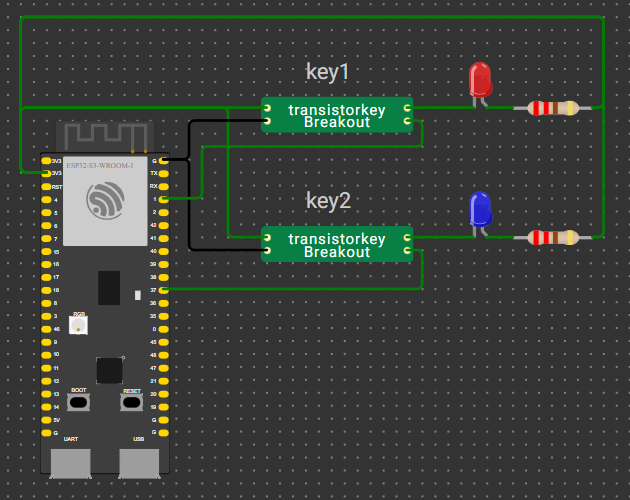
\includegraphics[width=0.8\textwidth]{scheme.png}
        \caption{\centering Схема транзисторних ключів для керування світлодіодами за допомогою плати esp32-s3}
    \end{figure}

    \noindent
    Що містить:

    \begin{itemize}
        \item Плату esp32-s3;
        \item 2 транзисторні ключі, які реалізовані за допомогою Custom Chip;
        \item 2 світлодіоди з відповідними резисторами обмеження струму (220 Ом);
    \end{itemize}

    \newpage

    \noindent
    \textbf{\underline{Arduino код для плати esp32-s3 (\texttt{sketch.ino}):}}

    \begin{minted}{cpp}
const int KEY1 = 1;  // GPIO1 -> IN першого ключа
const int KEY2 = 37; // GPIO37 -> IN другого ключа

void setup() {
  pinMode(KEY1, OUTPUT);
  pinMode(KEY2, OUTPUT);

  digitalWrite(KEY1, LOW); // ключі закриті, LEDи вимкнені
  digitalWrite(KEY2, LOW);
}

void loop() {
  // LED1 (червоний)
  digitalWrite(KEY1, HIGH); // відкриваємо ключ №1
  delay(500);
  digitalWrite(KEY1, LOW);  // закриваємо ключ №1
  delay(500);

  // LED2 (синій)
  digitalWrite(KEY2, HIGH); // відкриваємо ключ №2
  delay(500);
  digitalWrite(KEY2, LOW);  // закриваємо ключ №2
  delay(500);
}
    \end{minted}

    \noindent
    \textbf{\underline{Опис транзисторного ключа (\texttt{transistorkey.chip.json}):}}

    \begin{minted}{json}
{
  "name": "transistorkey",
  "author": "Artem Davydchuk",
  "pins": [
    "VCC",
    "GND",
    "IN",
    "OUT"
  ],
  "controls": []
}
    \end{minted}

    \noindent
    \textbf{\underline{Код реалізації транзисторного ключа (\texttt{transistorkey.chip.c}):}}

    \begin{minted}{c}
// Transistor Key
// IN = HIGH  -> OUT = LOW  (ключ відкритий, LED світиться)
// IN = LOW   -> OUT = HIGH (ключ закритий, LED вимкнений)

#include "wokwi-api.h"
#include <stdlib.h>

typedef struct {
  pin_t pin_in;
  pin_t pin_out;
} chip_state_t;

static void chip_pin_change(void *user_data, pin_t pin, uint32_t value) {
  chip_state_t *chip = (chip_state_t *)user_data;

  if (pin == chip->pin_in) {
    if (value == HIGH) {
      // Відкриваємо ключ
      pin_write(chip->pin_out, LOW);
    } else {
      // Закриваємо ключ
      pin_write(chip->pin_out, HIGH);
    }
  }
}

void chip_init(void) {
  chip_state_t *chip = malloc(sizeof(chip_state_t));

  chip->pin_in  = pin_init("IN",  INPUT);
  chip->pin_out = pin_init("OUT", OUTPUT_HIGH); // стартово LED вимкнений

  const pin_watch_config_t config = {
    .edge       = BOTH,
    .pin_change = chip_pin_change,
    .user_data  = chip,
  };

  pin_watch(chip->pin_in, &config);
}
    \end{minted}

    \noindent
    Весь проект можна знайти за посиланням: \href{https://wokwi.com/projects/449961857033405441}{Проект на Wokwi}.

    \vspace{1em}

    \noindent
    Демонстрація роботи схеми у 2 станах:

    \begin{figure}[h]
        \centering
        
        \begin{subfigure}[t]{0.48\textwidth}
            \centering
            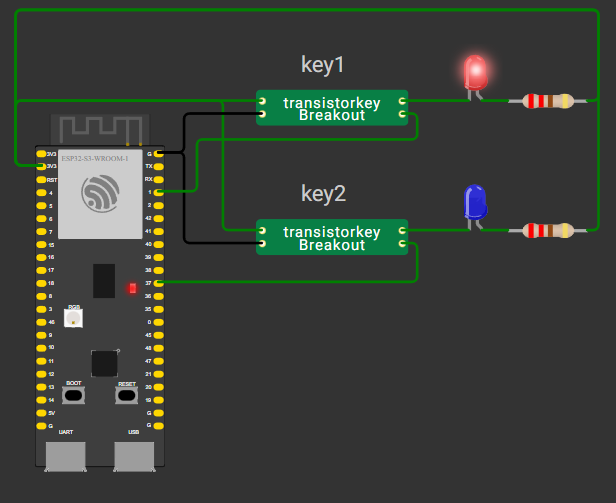
\includegraphics[width=\linewidth]{test1.png} % перше фото
            \caption{\centering 1 ключ відкритий, червоний світлодіод світиться}
        \end{subfigure}
        \hfill
        \begin{subfigure}[t]{0.48\textwidth}
            \centering
            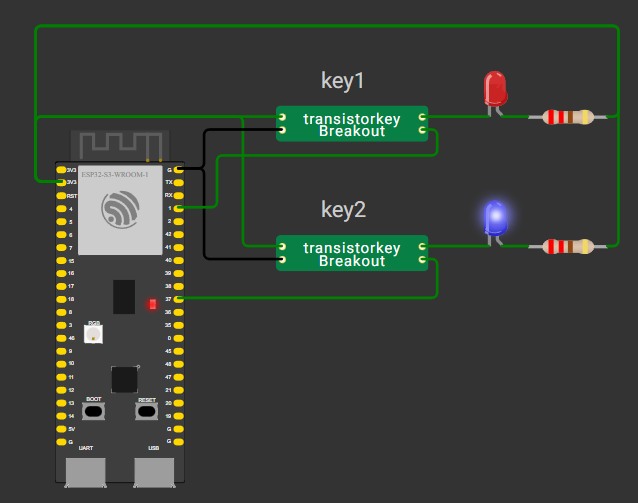
\includegraphics[width=\linewidth]{test2.png} % друге фото
            \caption{\centering 2 ключ відкритий, синій світлодіод світиться}
        \end{subfigure}
        \caption{Демонстрація роботи схеми}

    \end{figure}

    \newpage

    \noindent
\textbf{\underline{Висновок:}} У ході роботи було реалізовано та протестовано два транзисторні ключі для керування світлодіодами за допомогою плати ESP32-S3. Логіку роботи ключів було створено у вигляді власного Custom Chip мовою~C, після чого побудовано повну схему та написано Arduino-код керування. У роботі ключі поводяться як NPN-транзистори: при подачі логічної ``1'' на вхід IN вихід OUT переходить у низький рівень, і світлодіод світиться; при логічному ``0'' ключ закривається, і світлодіод гасне. Для обмеження струму через світлодіоди були використані резистори 220~Ом, що забезпечує коректний робочий режим та запобігає їх пошкодженню. Кожен сигнал триває 500~мс, так само як і пауза між ним.

Схема працює коректно, тому поставлену мету виконано.

\end{document}